\documentclass[10pt,t]{beamer}

% fonts
\usefonttheme{professionalfonts}
\usepackage[osf, sc]{mathpazo} % for rm
\usepackage{courier} % for mono
% \usepackage[euler-digits]{eulervm}
\usefonttheme{serif}
% more about eulervm:
% \mathrm -> rmdefault
% \mathbf -> bfdefault
% \mathsf -> sfdefault
% \mathtt -> ttdefault
% Thus, you should redefine the default text fonts before loading the eulervm package!
% redefine: \mathit, \mathbold, \mathcal

%math
\usepackage{amsmath}
\DeclareMathOperator*{\argmin}{arg\,min}
\DeclareMathOperator*{\argmax}{arg\,max}
\newcommand*\diff{\mathop{}\!\mathrm{d}}
% color
\definecolor{brown}{rgb}{0.4, 0.208, 0.192}
\definecolor{gray1}{rgb}{0.125, 0.125, 0.125}
\definecolor{gray2}{rgb}{0.157, 0.157, 0.157}
\definecolor{green2}{rgb}{0.16862745098039217,0.4,0.19607843137254902}
\definecolor{blue2}{rgb}{0,0.40784313725490196,0.6352941176470588}
\definecolor{brown2}{rgb}{0.6235294117647059,0.2901960784313726,0}

\definecolor{blue}{rgb}{0.18, 0.2, 0.529}
\definecolor{orange}{RGB}{206,117,59} % used for strong
\definecolor{green}{RGB}{49,104,108} % used for everywhere, link,...
\definecolor{red}{RGB}{133,60,66}
\definecolor{pink}{RGB}{184,86,150}



\setbeamercolor{caption name}{fg=green}

% settings for itemize and enumerate
\setbeamertemplate{itemize item}{\textbullet}
\setbeamertemplate{itemize subitem}{\bfseries --}
\setbeamertemplate{itemize subsubitem}{$\circ$}
\setbeamercolor{itemize item}{fg=green}
\setbeamercolor{itemize subitem}{fg=brown}
\setbeamercolor{itemize subsubitem}{fg=gray2}

\setbeamertemplate{enumerate item}{\arabic{enumi}.}
\setbeamertemplate{enumerate subitem}{(\roman{enumii})}
\setbeamertemplate{enumerate subsubitem}{\alph{enumiii}.}
\setbeamercolor{enumerate item}{fg=green}
\setbeamercolor{enumerate subitem}{fg=brown}
\setbeamercolor{enumerate subsubitem}{fg=gray2}
% main page style
\setbeamercolor{background canvas}{bg=white}
\setbeamercolor{normal text}{fg=black}
\setbeamertemplate{footline}[frame number]
\setbeamertemplate{navigation symbols}{}
\setbeamercolor{block title}{bg=green!90!black,fg=white}
\setbeamercolor{block body}{bg=green!10}
% frametitle
\setbeamertemplate{frametitle}
{
    \vskip 5pt
    \strut\Large\textcolor{green}{\insertframetitle}\strut
    \ifx\insertframesubtitle\empty
    \vskip-1.7ex
    \textcolor{green}{\hrule height0pt depth0.5pt \relax}
    \else
    \vskip-1ex
    \strut\small\textcolor{green}{\insertframesubtitle}\strut
    \textcolor{green}{\hrule height0pt depth0.5pt \relax}
    \fi
}
% titlepage
\setbeamertemplate{title page}
{
  \makebox[\textwidth][c]{
    \begin{minipage}[b][0.75\paperheight][c]{0.9\textwidth}
      \centering
      \huge\rm\inserttitle\\
      \Large\rm\insertsubtitle
      \vskip-1.5ex
      \textcolor{green}{\hrule height0pt depth0.8pt \relax}
      \vskip5pt
      \rm\normalsize\insertauthor
    \end{minipage}
  }

  \makebox[\textwidth][c]{
    \begin{minipage}[b][0.25\paperheight][c]{0.4\textwidth}
      \centering
      \rm\insertinstitute
      \par
      \rm\insertdate
    \end{minipage}
  }
}

\usepackage{hyperref}

% dashed underline
\usepackage{ulem}

\usepackage{booktabs}
% ********************************************************************
% tikz
% ********************************************************************
\usepackage{tikz}
\usetikzlibrary{positioning}
\usetikzlibrary{decorations.markings}
\usepackage{pgfplots}






\title{Empirical Asset Pricing \\ Problem Set $4$}
\author{Yu Zhou, HKUST}
\date{\today}


\begin{document}

\maketitle

\begin{frame}{Use GMM to estimate CCAMP}
The model is
$$
E_t[(C_{t+1} / C_t)^{-\gamma} R_{t+1}^e] = 0
$$
Considering five excess returns:
\begin{itemize}
	\item rmrf
	\item smb
	\item hml
	\item rmw: robust operating profitability portfolios minus weak operating profitability portfolios;
	\item cma: conservative investment portfolios minus aggresive investment portfolios.
\end{itemize}
\end{frame}


\begin{frame}{Q1: Descriptive statistics}
\begin{table}
\begin{tabular}{lcccccc}
\toprule
 & $C_{t+1} / C_{t}$ & rmrf & smb & hml & rmw & cma \\
\cmidrule{1-7}
mean & $102.28\%$ & $6.78\%$ & $3.36\%$ & $4.66\%$ & $3.64\%$ & $3.70\%$ \\
std & $1.37\%$ & $17.53\%$ & $12.87\%$ & $16.13\%$ & $12.77\%$ & $9.06\%$ \\
SR & & $0.39$ & $0.26$ & $0.29$ & $0.29$ & $0.41$ \\
\cmidrule{1-7}
corr &&&&&& \\
$C_{t+1} / C_{t}$ & & $0.20$ & $0.10$ & $0.11$ & $-0.12$ & $-0.11$ \\
rmrf & & & $0.23$ & $-0.14$ & $-0.38$ & $-0.28$ \\
smb &&&& $-0.10$ & $-0.42$ & $-0.02$ \\
hml &&&&& $0.36$ & $0.74$ \\
rmw &&&&&& $0.22$ \\
cma &&&&&& \\
\bottomrule
\end{tabular}
\caption{The consumption growth is positively correlated with rmrf, smb and hml, but negatively correlated with rmw and cma. The market excess return has the highest correlation with the consumption growth.}
\end{table}
\end{frame}



\begin{frame}{Q2: The equity premium puzzle}
\begin{figure}[h!]
\centering
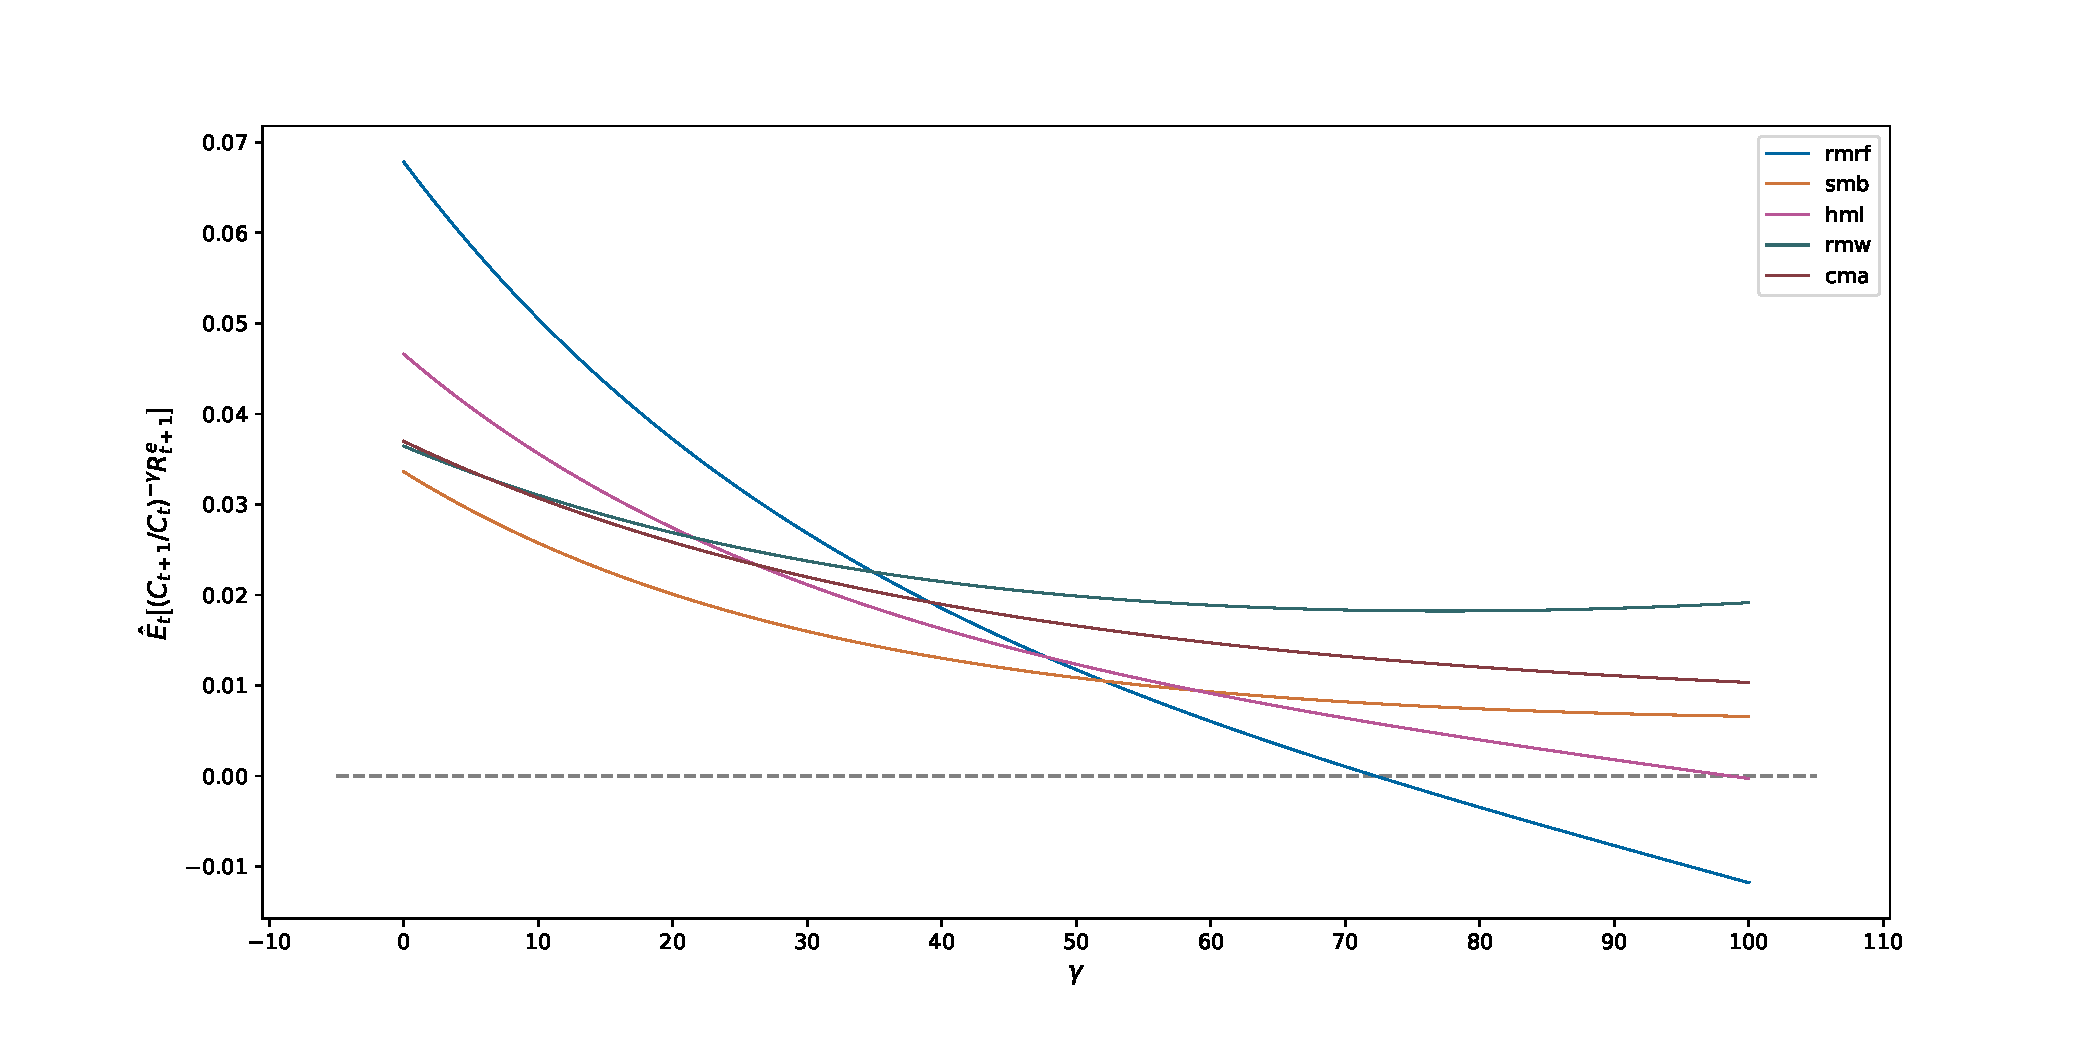
\includegraphics[width=\linewidth]{q2fig1.pdf}
\caption{The price of excess return rmrf crosses zero around $\gamma = 72$, which features the risk premium puzzle. The line of hml crosses zero around $\gamma = 98$ which is higher than $72$ because the correlation between $C_{t+1} / C_t$ and hml is smaller. The other three never cross zero.}
\end{figure}
\end{frame}


\begin{frame}{Q3: GMM}
\begin{table}
\begin{tabular}{lccc}
\toprule
& rmrf & smb & hml \\
\cmidrule{1-4}
\multicolumn{4}{l}{first-stage GMM} \\
$\gamma$ & $72.25$ & $116.59$ & $98.66$\\
$\sigma(\gamma)$ & $48.79$ & $1.08 \times 10^{11}$ & $63.53$\\
$\chi^2$ & - & - & - \\
$p$-value & - & - & - \\
$E(MR^e)$ & $0$ & $0.0064$ & $0$ \\
$\sigma(E(MR^e))$ & $0$ & $0$ & $0$ \\
$E(R^e)$ & $6.78\%$ & $3.36\%$ & $4.66\%$\\
$a\times 1000$ & $-0.4$ & $0$ & $-0.2$ \\
\bottomrule
\end{tabular}
\caption{In the first-stage GMM, $W = I$. When using rmrf and hml alone, we obtain high $\hat{\gamma}$ which are insignificant. When using smb alone, there does not exist any $\gamma$ making $g_T(\gamma) = 0$. So GMM sets $a_T = 0$. This result is meaningless.}
\end{table}
\end{frame}


\begin{frame}{Q3: GMM (cont'd)}
\begin{table}
\begin{tabular}{lccc}
\toprule
& rmrf & smb & hml \\
\cmidrule{1-4}
\multicolumn{4}{l}{second-stage GMM} \\
$\gamma$ & $72.25$ & $116.59$ & $98.66$\\
$\sigma(\gamma)$ & $48.79$ & $1.1 \times 10^{11}$ & $63.53$\\
$\chi^2$ & - & - & - \\
$p$-value & - & - & - \\
$E(MR^e)$ & $0$ & $0.0064$ & $0$ \\
$\sigma(E(MR^e))$ & $0$ & $0$ & $0$ \\
$E(R^e)$ & $6.78\%$ & $3.36\%$ & $4.66\%$\\
$a\times 1000$ & $-16.6$ & $0$ & $-22$ \\
\bottomrule
\end{tabular}
\caption{In the second-stage GMM, $W = \hat{S}_{\text{First Stage}}$. Compared with the first-stage GMM, the absolute weight on sample moment increases.}
\end{table}
\end{frame}


\begin{frame}{Q3: GMM (cont'd)}
\begin{table}
\begin{tabular}{lcccc}
\toprule
& rmrf & smb & rmrf & hml \\
\cmidrule{1-5}
\multicolumn{5}{l}{first-stage GMM} \\
$\gamma$ & $75.16$ &  & $77.6$ & \\
$\sigma(\gamma)$ & $49.68$ & & $42.85$ & \\
$\chi^2$ & $1.69$ & $0.19$ & $0.28$ & $0.6$ \\
$E(MR^e)$ & $-0.13\%$ & $0.78\%$ & $-0.24\%$ & $0.45\%$\\
$\sigma(E(MR^e))$ & $0.001$ & $0.006$ & $0.007$ & $0.013$\\
$E(R^e)$ & $6.78\%$ & $3.36\%$ & $6.78\%$ & $4.66\%$\\
$a\times 1000$ & $-0.45$ & $-0.077$ & $-0.44$ & $-0.23$\\
\bottomrule
\end{tabular}
\caption{The pricing errors are not zero. J-test fails to reject the null.}
\end{table}
\end{frame}

\begin{frame}{Q3: GMM (cont'd)}
\begin{table}
\begin{tabular}{lcccc}
\toprule
& rmrf & smb & rmrf & hml \\
\cmidrule{1-5}
\multicolumn{5}{l}{second-stage GMM} \\
$\gamma$ & $97$ &  & $85.27$ & \\
$\sigma(\gamma)$ & $62.54$ & & $40.45$ & \\
$\chi^2$ & $2.18$ & $0.14$ & $0$ & $1$ \\
$E(MR^e)$ & $-1.06\%$ & $0.67\%$ & $-0.57\%$ & $0.28\%$\\
$\sigma(E(MR^e))$ & $0.007$ & $0.004$ & $0.017$ & $0.009$ \\
$E(R^e)$ & $6.78\%$ & $3.36\%$ & $6.78\%$ & $4.66\%$\\
$a\times 1000$ & $-14.12$ & $-22.37$ & $-14.03$ & $-28.41$ \\
\bottomrule
\end{tabular}
\caption{The pricing errors are not zero. J-test fails to reject the null.}
\end{table}
\end{frame}











\begin{frame}{Q4: Conceptual questions}
(a)
\begin{itemize}
	\item The beta pricing formula always holds when the tangency portfolio is taken to be the reference.
	$$
	E[R_i] - R_f = \beta_{i,TAN} (E[R_{TAN}] - R_f)
	$$
	\item The beta pricing formula fails to hold when the value-weighted market portfolio is taken to be the reference, because investors have preference for those ``lottery-like'' stocks instead of purely mean-variance preference.
	$$
	E[R_i] - R_f = \beta_{i,MKT} (E[R_{MKT}] - R_f)
	$$
\end{itemize}
\end{frame}


\begin{frame}{Q4: Conceptual questions (cont'd)}
(b)
\begin{itemize}
	\item If the asset pricing model works well to explain expected return (that is to say the SDF lies in the factor span), then the intercept $a_i$ should be $0$.
	\item $R^2$ is not important because the objective of this model is to explain expected returns instead of realized returns.
	\item Low t-statistic for $b_i$ doesn't mean the model is wrong. When one asset's return is close to risk-free, it should have low risk loading (i.e., small $b_i$ that is insignificantly different from $0$). What we really care about is whether $a_i$ equal to $0$.
\end{itemize}
\end{frame}


\begin{frame}{Q4: Conceptual questions (cont'd)}
(c)
\begin{itemize}
	\item We can not evaluate this asset pricing model because $a_i$ is no longer the pricing error. $R^2$ is also not important because the objective of this model is to explain expected returns instead of realized returns.
\end{itemize}
\end{frame}

\begin{frame}{Q4: Conceptual questions (cont'd)}
(d)
\begin{itemize}
	\item For a good asset pricing model, $a_i$ should be $0$, $b_i$ should be the risk premium of the factors, and $R^2$ should be large as this model tries to explain expected returns.
\end{itemize}
\end{frame}

\begin{frame}{Q4: Conceptual questions (cont'd)}
(e)
\begin{itemize}
	\item For a good asset pricing model, $c_i$ should be $0$.
	\item It is acceptable to include $X_i^2$ and test the model.
	\item It is not acceptable to include $\beta_i^2$ because
	\begin{itemize}
		\item The model predicts a linear relationship between the expected excess returns and factor loadings. So the coefficient of $\beta_i^2$ is not meaningful;
		\item Including $\beta_i^2$ may make $b_i$ estimates less accurate.
	\end{itemize}
\end{itemize}
\end{frame}



\end{document}

